\documentclass{standalone}
\usepackage{tikz}
\usetikzlibrary{patterns, positioning}


\begin{document}
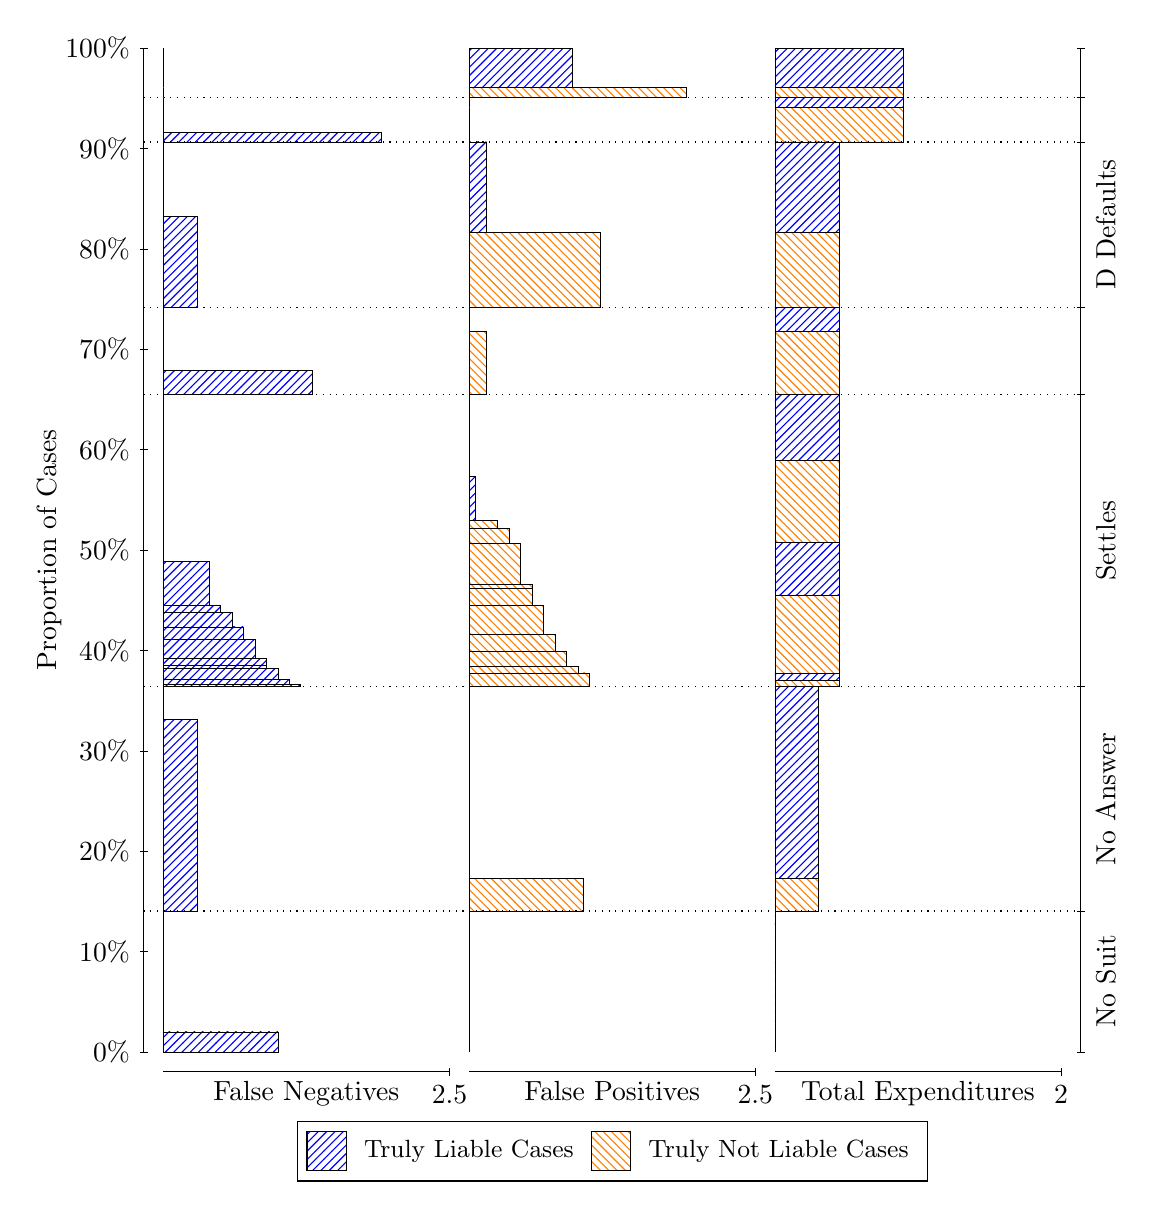
\begin{tikzpicture}
\draw[black, very thin] (1.5,1.75) -- (1.5,14.5);
\node[rotate=90, text=black, anchor=center] at (0.3, 8.125) {Proportion of Cases};
\draw[black, very thin] (1.45,1.75) -- (1.55,1.75);
\node[text=black, anchor=east] at (1.45, 1.75) {0\%};
\draw[black, very thin] (1.45,3.025) -- (1.55,3.025);
\node[text=black, anchor=east] at (1.45, 3.025) {10\%};
\draw[black, very thin] (1.45,4.3) -- (1.55,4.3);
\node[text=black, anchor=east] at (1.45, 4.3) {20\%};
\draw[black, very thin] (1.45,5.575) -- (1.55,5.575);
\node[text=black, anchor=east] at (1.45, 5.575) {30\%};
\draw[black, very thin] (1.45,6.85) -- (1.55,6.85);
\node[text=black, anchor=east] at (1.45, 6.85) {40\%};
\draw[black, very thin] (1.45,8.125) -- (1.55,8.125);
\node[text=black, anchor=east] at (1.45, 8.125) {50\%};
\draw[black, very thin] (1.45,9.4) -- (1.55,9.4);
\node[text=black, anchor=east] at (1.45, 9.4) {60\%};
\draw[black, very thin] (1.45,10.675) -- (1.55,10.675);
\node[text=black, anchor=east] at (1.45, 10.675) {70\%};
\draw[black, very thin] (1.45,11.95) -- (1.55,11.95);
\node[text=black, anchor=east] at (1.45, 11.95) {80\%};
\draw[black, very thin] (1.45,13.225) -- (1.55,13.225);
\node[text=black, anchor=east] at (1.45, 13.225) {90\%};
\draw[black, very thin] (1.45,14.5) -- (1.55,14.5);
\node[text=black, anchor=east] at (1.45, 14.5) {100\%};

\draw[black, very thin] (13.4,1.75) -- (13.4,14.5);
\draw[black, very thin] (13.35,1.75) -- (13.45,1.75);
\node[anchor=west] at (13.35, 1.75) {};
\draw[black, very thin] (13.35,3.5406) -- (13.45,3.5406);
\node[anchor=west] at (13.35, 3.5406) {};
\draw[black, very thin] (13.35,6.3884) -- (13.45,6.3884);
\node[anchor=west] at (13.35, 6.3884) {};
\draw[black, very thin] (13.35,10.098) -- (13.45,10.098);
\node[anchor=west] at (13.35, 10.098) {};
\draw[black, very thin] (13.35,11.21) -- (13.45,11.21);
\node[anchor=west] at (13.35, 11.21) {};
\draw[black, very thin] (13.35,13.307) -- (13.45,13.307);
\node[anchor=west] at (13.35, 13.307) {};
\draw[black, very thin] (13.35,13.87) -- (13.45,13.87);
\node[anchor=west] at (13.35, 13.87) {};
\draw[black, very thin] (13.35,14.5) -- (13.45,14.5);
\node[anchor=west] at (13.35, 14.5) {};

\draw[black, very thin, pattern color=blue, pattern=north east lines] (1.75,1.75) rectangle (3.2033,2.0064);
\draw[black, very thin, pattern color=orange, pattern=north west lines] (1.75,2.0064) rectangle (1.75,3.5406);
\draw[black, very thin, pattern color=blue, pattern=north east lines] (1.75,3.5406) rectangle (2.186,5.9784);
\draw[black, very thin, pattern color=orange, pattern=north west lines] (1.75,5.9784) rectangle (1.75,6.3884);
\draw[black, very thin, pattern color=blue, pattern=north east lines] (1.75,6.3884) rectangle (3.494,6.4222);
\draw[black, very thin, pattern color=blue, pattern=north east lines] (1.75,6.4222) rectangle (3.3487,6.4776);
\draw[black, very thin, pattern color=blue, pattern=north east lines] (1.75,6.4776) rectangle (3.2033,6.624);
\draw[black, very thin, pattern color=blue, pattern=north east lines] (1.75,6.624) rectangle (3.058,6.6664);
\draw[black, very thin, pattern color=blue, pattern=north east lines] (1.75,6.6664) rectangle (3.058,6.7513);
\draw[black, very thin, pattern color=blue, pattern=north east lines] (1.75,6.7513) rectangle (2.9127,6.9869);
\draw[black, very thin, pattern color=blue, pattern=north east lines] (1.75,6.9869) rectangle (2.7673,7.1482);
\draw[black, very thin, pattern color=blue, pattern=north east lines] (1.75,7.1482) rectangle (2.622,7.3336);
\draw[black, very thin, pattern color=blue, pattern=north east lines] (1.75,7.3336) rectangle (2.4767,7.4264);
\draw[black, very thin, pattern color=blue, pattern=north east lines] (1.75,7.4264) rectangle (2.3313,7.982);
\draw[black, very thin, pattern color=orange, pattern=north west lines] (1.75,7.982) rectangle (1.75,10.098);
\draw[black, very thin, pattern color=blue, pattern=north east lines] (1.75,10.098) rectangle (3.6393,10.404);
\draw[black, very thin, pattern color=orange, pattern=north west lines] (1.75,10.404) rectangle (1.75,11.21);
\draw[black, very thin, pattern color=blue, pattern=north east lines] (1.75,11.21) rectangle (2.186,12.361);
\draw[black, very thin, pattern color=orange, pattern=north west lines] (1.75,12.361) rectangle (1.75,13.307);
\draw[black, very thin, pattern color=blue, pattern=north east lines] (1.75,13.307) rectangle (4.5113,13.433);
\draw[black, very thin, pattern color=orange, pattern=north west lines] (1.75,13.433) rectangle (1.75,13.87);
\draw[black, very thin, pattern color=orange, pattern=north west lines] (1.75,13.87) rectangle (1.75,13.996);
\draw[black, very thin, pattern color=blue, pattern=north east lines] (1.75,13.996) rectangle (1.75,14.5);
\draw[black, very thin, pattern color=orange, pattern=north west lines] (5.6333,1.75) rectangle (5.6333,3.2842);
\draw[black, very thin, pattern color=blue, pattern=north east lines] (5.6333,3.2842) rectangle (5.6333,3.5406);
\draw[black, very thin, pattern color=orange, pattern=north west lines] (5.6333,3.5406) rectangle (7.0867,3.9507);
\draw[black, very thin, pattern color=blue, pattern=north east lines] (5.6333,3.9507) rectangle (5.6333,6.3884);
\draw[black, very thin, pattern color=orange, pattern=north west lines] (5.6333,6.3884) rectangle (7.1593,6.5641);
\draw[black, very thin, pattern color=orange, pattern=north west lines] (5.6333,6.5641) rectangle (7.014,6.6456);
\draw[black, very thin, pattern color=orange, pattern=north west lines] (5.6333,6.6456) rectangle (6.8687,6.8377);
\draw[black, very thin, pattern color=orange, pattern=north west lines] (5.6333,6.8377) rectangle (6.7233,7.0531);
\draw[black, very thin, pattern color=orange, pattern=north west lines] (5.6333,7.0531) rectangle (6.578,7.4254);
\draw[black, very thin, pattern color=orange, pattern=north west lines] (5.6333,7.4254) rectangle (6.4327,7.637);
\draw[black, very thin, pattern color=orange, pattern=north west lines] (5.6333,7.637) rectangle (6.4327,7.6875);
\draw[black, very thin, pattern color=orange, pattern=north west lines] (5.6333,7.6875) rectangle (6.2873,8.2053);
\draw[black, very thin, pattern color=orange, pattern=north west lines] (5.6333,8.2053) rectangle (6.142,8.399);
\draw[black, very thin, pattern color=orange, pattern=north west lines] (5.6333,8.399) rectangle (5.9967,8.5043);
\draw[black, very thin, pattern color=blue, pattern=north east lines] (5.6333,8.5043) rectangle (5.706,9.0598);
\draw[black, very thin, pattern color=blue, pattern=north east lines] (5.6333,9.0598) rectangle (5.6333,10.098);
\draw[black, very thin, pattern color=orange, pattern=north west lines] (5.6333,10.098) rectangle (5.8513,10.904);
\draw[black, very thin, pattern color=blue, pattern=north east lines] (5.6333,10.904) rectangle (5.6333,11.21);
\draw[black, very thin, pattern color=orange, pattern=north west lines] (5.6333,11.21) rectangle (7.3047,12.156);
\draw[black, very thin, pattern color=blue, pattern=north east lines] (5.6333,12.156) rectangle (5.8513,13.307);
\draw[black, very thin, pattern color=orange, pattern=north west lines] (5.6333,13.307) rectangle (5.6333,13.743);
\draw[black, very thin, pattern color=blue, pattern=north east lines] (5.6333,13.743) rectangle (5.6333,13.87);
\draw[black, very thin, pattern color=orange, pattern=north west lines] (5.6333,13.87) rectangle (8.3947,13.996);
\draw[black, very thin, pattern color=blue, pattern=north east lines] (5.6333,13.996) rectangle (6.9413,14.5);
\draw[black, very thin, pattern color=orange, pattern=north west lines] (9.5167,1.75) rectangle (9.5167,3.2842);
\draw[black, very thin, pattern color=blue, pattern=north east lines] (9.5167,3.2842) rectangle (9.5167,3.5406);
\draw[black, very thin, pattern color=orange, pattern=north west lines] (9.5167,3.5406) rectangle (10.062,3.9507);
\draw[black, very thin, pattern color=blue, pattern=north east lines] (9.5167,3.9507) rectangle (10.062,6.3884);
\draw[black, very thin, pattern color=orange, pattern=north west lines] (9.5167,6.3884) rectangle (10.334,6.4699);
\draw[black, very thin, pattern color=blue, pattern=north east lines] (9.5167,6.4699) rectangle (10.334,6.5628);
\draw[black, very thin, pattern color=orange, pattern=north west lines] (9.5167,6.5628) rectangle (10.334,7.5542);
\draw[black, very thin, pattern color=blue, pattern=north east lines] (9.5167,7.5542) rectangle (10.334,8.2214);
\draw[black, very thin, pattern color=orange, pattern=north west lines] (9.5167,8.2214) rectangle (10.334,9.2643);
\draw[black, very thin, pattern color=blue, pattern=north east lines] (9.5167,9.2643) rectangle (10.334,10.098);
\draw[black, very thin, pattern color=orange, pattern=north west lines] (9.5167,10.098) rectangle (10.334,10.904);
\draw[black, very thin, pattern color=blue, pattern=north east lines] (9.5167,10.904) rectangle (10.334,11.21);
\draw[black, very thin, pattern color=orange, pattern=north west lines] (9.5167,11.21) rectangle (10.334,12.156);
\draw[black, very thin, pattern color=blue, pattern=north east lines] (9.5167,12.156) rectangle (10.334,13.307);
\draw[black, very thin, pattern color=orange, pattern=north west lines] (9.5167,13.307) rectangle (11.152,13.743);
\draw[black, very thin, pattern color=blue, pattern=north east lines] (9.5167,13.743) rectangle (11.152,13.87);
\draw[black, very thin, pattern color=orange, pattern=north west lines] (9.5167,13.87) rectangle (11.152,13.996);
\draw[black, very thin, pattern color=blue, pattern=north east lines] (9.5167,13.996) rectangle (11.152,14.5);
\draw[black, dotted] (1.5,3.5406) -- (13.4,3.5406);
\draw[black, dotted] (1.5,6.3884) -- (13.4,6.3884);
\draw[black, dotted] (1.5,10.098) -- (13.4,10.098);
\draw[black, dotted] (1.5,11.21) -- (13.4,11.21);
\draw[black, dotted] (1.5,13.307) -- (13.4,13.307);
\draw[black, dotted] (1.5,13.87) -- (13.4,13.87);
\draw[black, very thin] (1.75,1.5) -- (5.3833,1.5);
\node[text=black, anchor=north] at (3.5667, 1.5) {False Negatives};
\draw[black, very thin] (5.3833,1.45) -- (5.3833,1.55);
\node[text=black, anchor=north] at (5.3833, 1.45) {2.5};

\draw[black, very thin] (5.6333,1.5) -- (9.2667,1.5);
\node[text=black, anchor=north] at (7.45, 1.5) {False Positives};
\draw[black, very thin] (9.2667,1.45) -- (9.2667,1.55);
\node[text=black, anchor=north] at (9.2667, 1.45) {2.5};

\draw[black, very thin] (9.5167,1.5) -- (13.15,1.5);
\node[text=black, anchor=north] at (11.333, 1.5) {Total Expenditures};
\draw[black, very thin] (13.15,1.45) -- (13.15,1.55);
\node[text=black, anchor=north] at (13.15, 1.45) {2};

\node[text=black, centered, rotate=90] at (13.72, 2.6453) {No Suit};
\node[text=black, centered, rotate=90] at (13.72, 4.9645) {No Answer};
\node[text=black, centered, rotate=90] at (13.72, 8.2431) {Settles};

\node[text=black, centered, rotate=90] at (13.72, 12.258) {D Defaults};



\draw (7.449999999999999,1.5) node[draw=none] (baseCoordinate) {};
\begin{scope}[align=center]
        \matrix[scale=0.5, draw=black, below=0.5cm of baseCoordinate, nodes={draw}, column sep=0.1cm]{
            \node[rectangle, draw, minimum width=0.5cm, minimum height=0.5cm, pattern color=blue, pattern=north east lines] {}; &
            \node[draw=none, font=\small, text=black] (B) {Truly Liable Cases}; &
            \node[rectangle, draw, minimum width=0.5cm, minimum height=0.5cm, pattern color=orange, pattern=north west lines] {}; &
            \node[draw=none, font=\small, text=black] (B) {Truly Not Liable Cases}; \\
            };
\end{scope}

\end{tikzpicture}
\end{document}